\documentclass[UTF8,zihao=-4]{ctexart}

% =========================================================
% 版式主题：EIC FPGA Tetris Report Style
% =========================================================
\usepackage[a4paper,left=2.35cm,right=2.35cm,top=2.65cm,bottom=2.45cm,headheight=36pt,headsep=0.55cm]{geometry}
\usepackage{amsmath,amssymb}
\usepackage{booktabs,longtable,tabularx,array,multirow}
\usepackage{xcolor}
\usepackage{graphicx}
\usepackage{float}
\usepackage{fancyhdr}
\usepackage{titlesec}
\usepackage[most]{tcolorbox}
\usepackage{listings}
\usepackage{caption}
\usepackage{subcaption}
\usepackage{hyperref}
\usepackage{enumitem}
\usepackage{tocloft}
\usepackage{indentfirst}
\usepackage{tikz}
\usetikzlibrary{shapes.geometric,arrows.meta,positioning,fit,calc,decorations.pathmorphing,shadows}
\setmonofont{DejaVu Sans Mono}

% =========================================================
% 颜色系统
% =========================================================
\definecolor{eicnavy}{HTML}{0A1633}
\definecolor{eicblue}{HTML}{1455D9}
\definecolor{eiccyan}{HTML}{16C8F7}
\definecolor{eicpurple}{HTML}{7C3AED}
\definecolor{eicgray}{HTML}{334155}
\definecolor{eiclight}{HTML}{F4F8FF}
\definecolor{eicline}{HTML}{C8D7F2}
\definecolor{codebg}{HTML}{F7F9FC}
\definecolor{codeframe}{HTML}{B8C7E6}
\definecolor{keyword}{HTML}{1648B8}
\definecolor{comment}{HTML}{15803D}
\definecolor{string}{HTML}{A21CAF}

\hypersetup{
    colorlinks=true,
    linkcolor=eicblue,
    urlcolor=eicblue,
    citecolor=eicblue,
    linktoc=all,
    pdftitle={基于 FPGA 的 VGA 俄罗斯方块交互游戏设计与实现},
    pdfauthor={424组}
}

% =========================================================
% 报告信息：后续只需改这里
% =========================================================
\newcommand{\reporttitle}{基于 FPGA 的 VGA 俄罗斯方块交互游戏设计与实现}
\newcommand{\covermaintitle}{基于 FPGA 的 VGA 俄罗斯方块\\交互游戏设计与实现}
\newcommand{\reportsubtitle}{FPGA Tetris VGA Edition}
\newcommand{\coursename}{微机原理实验 / FPGA 综合设计}
\newcommand{\classname}{请填写班级}
\newcommand{\teammembers}{424组（请填写成员姓名与学号）}
\newcommand{\experimentdate}{\today}
\newcommand{\instructor}{请填写指导教师}
\newcommand{\boardinfo}{Nexys4 DDR · Artix-7 · Vivado 2018.3 · Verilog-2001}
\setlength{\parindent}{2em}
\setlength{\parskip}{0.25em}

% =========================================================
% Logo 命令：请将 logo.jpg 放在 tex 同目录
% =========================================================
\newcommand{\reportlogo}[1][1.0cm]{%
  \IfFileExists{local_report_files/logo.jpg}{%
    
\includegraphics[height=#1]{local_report_files/logo.jpg}%
  }{%
    \IfFileExists{logo.jpg}{%
      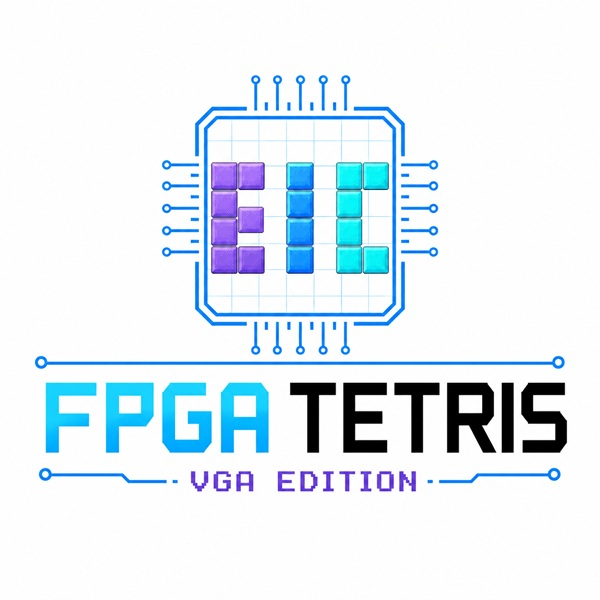
\includegraphics[height=#1]{logo.jpg}%
    }{%
      \textcolor{eicblue}{\fbox{\bfseries EIC}}%
    }%
  }%
}

% =========================================================
% 页眉页脚：每页右上角 Logo
% =========================================================
\pagestyle{fancy}
\fancyhf{}
\fancyhead[L]{\small\textcolor{eicgray}{\reportsubtitle}}
\fancyhead[C]{\small\textcolor{eicblue}{\coursename}}
\fancyhead[R]{\reportlogo[1.08cm]}
\fancyfoot[L]{\small\textcolor{eicgray}{424组}}
\fancyfoot[C]{\small\textcolor{eicgray}{第 \thepage 页}}
\fancyfoot[R]{\small\textcolor{eicgray}{VGA 俄罗斯方块}}
\renewcommand{\headrulewidth}{0.6pt}
\renewcommand{\footrulewidth}{0.4pt}
\renewcommand{\headrule}{\hbox to\headwidth{\color{eicline}\leaders\hrule height \headrulewidth\hfill}}
\renewcommand{\footrule}{\hbox to\headwidth{\color{eicline}\leaders\hrule height \footrulewidth\hfill}}

\fancypagestyle{plain}{%
  \fancyhf{}%
  \fancyhead[L]{\small\textcolor{eicgray}{\reportsubtitle}}%
  \fancyhead[C]{\small\textcolor{eicblue}{\coursename}}%
  \fancyhead[R]{\reportlogo[1.08cm]}%
  \fancyfoot[L]{\small\textcolor{eicgray}{424组}}%
  \fancyfoot[C]{\small\textcolor{eicgray}{第 \thepage 页}}%
  \fancyfoot[R]{\small\textcolor{eicgray}{VGA 俄罗斯方块}}%
  \renewcommand{\headrulewidth}{0.6pt}%
  \renewcommand{\footrulewidth}{0.4pt}%
}

% =========================================================
% 标题、目录、列表样式
% =========================================================
\titleformat{\section}
  {\Large\heiti\bfseries\color{eicnavy}}
  {\tikz[baseline=(n.base)]\node[fill=eicblue,text=white,rounded corners=2pt,inner xsep=6pt,inner ysep=3pt](n){\thesection};}
  {0.8em}{}
\titleformat{\subsection}
  {\large\heiti\bfseries\color{eicblue}}
  {\thesubsection}{0.75em}{}
\titleformat{\subsubsection}
  {\normalsize\heiti\bfseries\color{eicgray}}
  {\thesubsubsection}{0.75em}{}
\titlespacing{\section}{0pt}{1.25em}{0.85em}
\titlespacing{\subsection}{0pt}{0.95em}{0.5em}
\titlespacing{\subsubsection}{0pt}{0.7em}{0.35em}

\setlist[itemize]{leftmargin=2em,itemsep=0.18em,topsep=0.35em}
\setlist[enumerate]{leftmargin=2em,itemsep=0.18em,topsep=0.35em}
\renewcommand{\cftsecfont}{\bfseries\color{eicnavy}}
\renewcommand{\cftsecpagefont}{\bfseries\color{eicnavy}}
\renewcommand{\cftsubsecfont}{\color{eicgray}}
\renewcommand{\cftsubsecpagefont}{\color{eicgray}}
\setlength{\cftbeforesecskip}{0.35em}
\renewcommand{\contentsname}{目录}
\renewcommand{\listfigurename}{图目录}

% =========================================================
% 图表与盒子
% =========================================================
\captionsetup{font=small,labelfont={bf,color=eicblue},textfont={color=eicgray}}
\renewcommand{\arraystretch}{1.18}
\newcolumntype{Y}{>{\raggedright\arraybackslash}X}

\newtcolorbox{abstractbox}{
  enhanced,
  colback=eiclight,
  colframe=eicblue,
  coltitle=white,
  title=\heiti 摘要与关键词,
  fonttitle=\bfseries,
  boxrule=0.9pt,
  arc=2mm,
  left=5mm,right=5mm,top=4mm,bottom=4mm,
  attach boxed title to top left={xshift=4mm,yshift=-2mm},
  boxed title style={colback=eicblue,arc=1.5mm,boxrule=0pt}
}

\newtcolorbox{infobox}[1]{
  enhanced,
  breakable,
  title=\textbf{#1},
  coltitle=white,
  colback=eiclight,
  colframe=eicblue,
  colbacktitle=eicblue,
  boxrule=0.8pt,
  arc=1.5mm,
  left=2mm,right=2mm,top=2mm,bottom=2mm
}

\newtcolorbox{teamdivisionbox}{
  enhanced,
  breakable,
  title=\heiti 团队成员分工,
  coltitle=white,
  colback=white,
  colframe=eicblue,
  colbacktitle=eicblue,
  boxrule=0.8pt,
  arc=1.5mm,
  left=4mm,right=4mm,top=3mm,bottom=3mm
}

\newcommand{\simwavefigure}[3]{%
  \IfFileExists{#1}{%
    \includegraphics[width=#2\textwidth]{#1}%
  }{%
    \IfFileExists{local_report_files/#1}{%
      \includegraphics[width=#2\textwidth]{local_report_files/#1}%
    }{%
      \fbox{\parbox[c][4cm][c]{#2\textwidth}{\centering #3\\（建议图片文件名：\texttt{\detokenize{#1}}）}}%
    }%
  }%
}

% =========================================================
% 代码块样式
% =========================================================
\lstdefinestyle{mycode}{
    backgroundcolor=\color{codebg},
    basicstyle=\ttfamily\small,
    breaklines=true,
    captionpos=b,
    keepspaces=true,
    numbers=left,
    numberstyle=\tiny\color{eicgray},
    showspaces=false,
    showstringspaces=false,
    showtabs=false,
    tabsize=4,
    frame=single,
    rulecolor=\color{codeframe},
    xleftmargin=1.2em,
    xrightmargin=1.2em,
    framexleftmargin=1.2em,
    framexrightmargin=1.2em,
    keywordstyle=\color{keyword}\bfseries,
    commentstyle=\color{comment}\itshape,
    stringstyle=\color{string},
    columns=fullflexible
}
\lstset{style=mycode}

\begin{document}
\begin{titlepage}
\thispagestyle{empty}
\begin{tikzpicture}[remember picture,overlay]
  \fill[eicnavy] (current page.north west) rectangle ([yshift=-6.15cm]current page.north east);
  \fill[eicblue] ([yshift=-6.15cm]current page.north west) -- ([yshift=-6.15cm]current page.north east) -- ([yshift=-6.72cm]current page.north east) -- ([yshift=-6.36cm]current page.north west) -- cycle;
  \foreach \x in {0.8,2.0,...,19.2}{\draw[eiccyan!28,line width=0.42pt] ([xshift=\x cm,yshift=-0.65cm]current page.north west) -- ++(0,-4.85cm);}
  \foreach \y in {-0.95,-1.75,...,-5.25}{\draw[eiccyan!20,line width=0.42pt] ([xshift=0.7cm,yshift=\y cm]current page.north west) -- ++(19.7cm,0);}
  \draw[eiccyan,line width=1.1pt] ([xshift=1.2cm,yshift=-5.25cm]current page.north west) -- ++(4.1cm,0) -- ++(0.35cm,-0.32cm) -- ++(3.8cm,0);
  \draw[eicpurple,line width=1.2pt] ([xshift=12.2cm,yshift=-1.1cm]current page.north west) -- ++(2.5cm,0) -- ++(0.4cm,0.4cm) -- ++(3.1cm,0);
  \node[anchor=north east,inner sep=0pt] at ([xshift=-1.35cm,yshift=-0.82cm]current page.north east) {\reportlogo[2.25cm]};
  \node[anchor=west,text=white,font=\bfseries\fontsize{25}{31}\selectfont] at ([xshift=1.45cm,yshift=-4.75cm]current page.north west) {\reportsubtitle};
  \node[anchor=west,text=eiccyan,font=\bfseries\fontsize{13}{18}\selectfont] at ([xshift=1.45cm,yshift=-6.95cm]current page.north west) {\boardinfo};
\end{tikzpicture}

\vspace*{8.0cm}
\begin{center}
  {\heiti\bfseries\color{eicnavy}\fontsize{24}{34}\selectfont \covermaintitle}\\[1.1cm]
  {\color{eicblue}\fontsize{18}{24}\selectfont 课程实验报告}\\[1.55cm]
\end{center}

\begin{center}
\begin{tcolorbox}[
  enhanced,
  colback=white,
  colframe=eicblue,
  boxrule=1.1pt,
  arc=2mm,
  width=0.76\textwidth,
  left=7mm,
  right=7mm,
  top=5mm,
  bottom=5mm
]
\renewcommand{\arraystretch}{1.65}
\begin{tabular}{>{\heiti\bfseries\color{eicnavy}}p{3.1cm} p{0.54\textwidth}}
实验名称 & \reporttitle \\
课程名称 & \coursename \\
班级 & \classname \\
实验成员 & \teammembers \\
指导教师 & \instructor \\
实验日期 & \experimentdate \\
\end{tabular}
\end{tcolorbox}
\end{center}

\vfill
\begin{center}
  {\small\color{eicgray}电子信息特色项目 · FPGA 硬件逻辑设计 · VGA 图形显示 · 交互式游戏系统}
\end{center}
\end{titlepage}
\pagestyle{fancy}

\begin{abstractbox}
\noindent 本文展示了一套基于 FPGA 的 VGA 俄罗斯方块交互游戏系统。系统使用 Digilent Nexys4 DDR 开发板，采用 Vivado 2018.3 和 Verilog-2001 完成硬件逻辑设计。项目通过模块化设计实现游戏核心、VGA显示、输入控制与外设反馈的解耦，重点展示了实现过程、调试优化、资源控制及阶段性上板成果。实验结果表明，系统能够完成俄罗斯方块主要游戏流程，支持方块移动、旋转、软降、消行、计分、等级管理、暂停/继续和 Game Over 后重新开始，并通过 VGA、LED 和数码管提供交互反馈。

\vspace{0.5cm}
\noindent \textbf{关键词：} FPGA；VGA；俄罗斯方块；状态机；资源优化；Verilog
\end{abstractbox}

\begin{teamdivisionbox}
\begin{tabularx}{\linewidth}{>{\heiti\bfseries\color{eicnavy}}p{2.2cm} Y}
成员A & 游戏核心逻辑设计，负责 \texttt{game\_core}、状态机、碰撞检测、消行、计分等级、资源优化与核心仿真。\\
成员B & VGA 显示与 UI 设计，负责 \texttt{vga\_timing}、\texttt{tetris\_video}、文字/数字显示、NEXT 预览、logo 显示与 VGA 上板调试。\\
成员C & 输入输出外设设计，负责 \texttt{button\_input}、\texttt{debounce}、\texttt{one\_pulse}、七段数码管、LED 状态与 Game Over 闪烁。\\
共同工作 & 系统集成、Vivado 综合实现、bitstream 生成、上板联调、Git 协作与文档整理。\\
\end{tabularx}
\end{teamdivisionbox}

\newpage
\tableofcontents
\newpage
\listoffigures
\newpage
% ================== 第1章：背景 ==================
\section{项目背景与设计目标}

\subsection{课题背景}
随着数字系统设计技术的发展，现场可编程门阵列（Field Programmable Gate Array，FPGA）凭借其高度并行、实时性强以及可重构等特点，被广泛应用于图像处理、工业控制、通信系统以及嵌入式系统等领域。与传统 MCU 或 CPU 软件实现方式不同，FPGA 可以利用硬件并行结构实现游戏逻辑和显示逻辑的同时运行，从而获得更高的实时性和更低的响应延迟。

俄罗斯方块（Tetris）是一款经典的实时交互式益智游戏，其运行过程涉及图形显示、用户输入、状态机控制、数据存储以及实时碰撞检测等多种数字系统设计内容，因此非常适合作为 FPGA 综合设计实验项目。通过 FPGA 实现俄罗斯方块游戏不仅能够验证数字逻辑设计能力，还能够深入理解状态机设计、模块化开发以及硬件资源优化方法。

\subsection{设计目标}
本项目基于 Digilent Nexys4 DDR FPGA 开发板实现一套完整的 VGA 俄罗斯方块交互游戏系统。
\begin{itemize}
    \item \textbf{显示方面：} 支持 VGA 640$\times$480 分辨率的实时图形输出。
    \item \textbf{游戏逻辑：} 实现标准 10$\times$20 棋盘和七种经典方块（I、O、T、S、Z、J、L），支持方块自动下落、左右移动、旋转和软降。
    \item \textbf{规则判定：} 实现精确的碰撞检测与边界检测。
    \item \textbf{流程控制：} 完成方块锁定、随机生成、满行检测与自动消行、分数统计与等级管理。
\end{itemize}

\subsection{系统需求分析}
系统运行过程中需要同时完成多项任务：用户输入采集需要在按键按下的瞬间产生有效信号；游戏逻辑状态更新需要在每个时钟周期内完成状态转移判断；VGA 像素需要按照严格的时序进行实时扫描输出；棋盘数据需要支持快速存储与随机访问；分数和等级需要根据消行结果实时计算；外设状态反馈需要与游戏进度保持同步。

由于上述任务在时间上存在严格的重叠关系，系统必须采用模块化结构，通过统一接口协议实现各模块之间的数据交互，才能保证各功能模块互不干扰、协同工作。

% ================== 第2章：顶层设计 ==================
\section{项目顶层设计}

\subsection{总体架构}
系统采用自顶向下（Top-Down）的设计思想，将整个俄罗斯方块系统划分为多个相互独立的功能模块。游戏核心模块（Game Core）作为系统控制中心，负责维护棋盘状态并向 VGA 提供显示数据；VGA 显示模块（VGA Renderer）根据当前状态实时渲染图像；输入控制模块（Button Input）负责按键消抖并产生控制事件；随机方块生成模块（LFSR）提供伪随机数以决定下一个方块类型；消行模块（Line Clear）负责满行检测与棋盘压缩；分数等级模块（Score Level）实时计算得分与等级；LED 与数码管显示模块则提供直观的状态反馈。

各模块通过统一接口协议进行通信，整个系统采用纯硬件实现方案，不依赖软核 CPU，因此所有游戏逻辑均由 FPGA 逻辑资源完成，充分发挥了 FPGA 并行处理的硬件优势。

\begin{figure}[H]
\centering
\resizebox{\textwidth}{!}{%
\begin{tikzpicture}[
  font=\small,
  module/.style={draw=eicblue,fill=eiclight,rounded corners=3pt,line width=0.8pt,minimum width=2.7cm,minimum height=0.85cm,align=center},
  core/.style={draw=eicnavy,fill=eicblue!10,rounded corners=4pt,line width=1.1pt,minimum width=4.5cm,minimum height=3.5cm,align=center},
  submodule/.style={draw=eiccyan!70!eicblue,fill=white,rounded corners=2pt,line width=0.6pt,minimum width=2.0cm,minimum height=0.56cm,align=center,font=\scriptsize},
  bus/.style={-Latex,line width=0.75pt,draw=eicblue},
  thinbus/.style={-Latex,line width=0.55pt,draw=eicgray}
]
  \node[module] (buttons) at (0,2.5) {BTNC/BTNU/BTND\\BTNL/BTNR};
  \node[module] (input) at (3.4,2.5) {\texttt{button\_input}\\消抖/单脉冲};
  \node[core] (core) at (7.5,1.0) {\large\heiti Game Core\\[2.3cm]};

  \node[submodule] (piece) at (6.15,1.75) {\texttt{piece\_rom}};
  \node[submodule] (rand)  at (8.85,1.75) {\texttt{random\_lfsr}};
  \node[submodule] (board) at (6.15,0.95) {board storage};
  \node[submodule] (coll)  at (8.85,0.95) {collision\\candidate check};
  \node[submodule] (lock)  at (6.15,0.12) {lock / clear FSM};
  \node[submodule] (score) at (8.85,0.12) {\texttt{score\_level}};

  \node[module] (video) at (12.1,2.35) {\texttt{tetris\_video}\\像素渲染/UI};
  \node[module] (timing) at (15.4,2.35) {\texttt{vga\_timing}\\640$\times$480};
  \node[module] (vgaout) at (18.8,2.35) {VGA\_R/G/B\\VGA\_HS/VGA\_VS};

  \node[module] (display) at (12.1,0.55) {\texttt{display}\\\texttt{seven\_seg\_driver}};
  \node[module] (segout) at (15.4,0.55) {\texttt{an[7:0]}\\\texttt{ca\_g[6:0]}};

  \node[module] (led) at (12.1,-1.15) {\texttt{led\_status}\\\texttt{led\_blink mux}};
  \node[module] (ledout) at (15.4,-1.15) {\texttt{LED[15:0]}};

  \node[module] (mem) at (12.1,4.0) {\texttt{logo\_128x128.mem}};
  \node[module] (rom) at (15.4,4.0) {\texttt{logo\_rom}};

  \draw[bus] (buttons) -- (input);
  \draw[bus] (input) -- node[above,font=\scriptsize]{start/left/right/rotate/soft drop} (core);
  \draw[bus] (core.east) -- node[above,font=\scriptsize]{board query + piece/state} (video.west);
  \draw[bus] (video) -- (timing);
  \draw[bus] (timing) -- (vgaout);
  \draw[bus] (core.east) |- node[pos=0.2,below,font=\scriptsize]{score / level} (display.west);
  \draw[bus] (display) -- (segout);
  \draw[bus] (core.east) |- node[pos=0.2,below,font=\scriptsize]{game\_state} (led.west);
  \draw[bus] (led) -- (ledout);
  \draw[thinbus] (mem) -- (rom);
  \draw[thinbus] (rom) |- node[pos=0.75,right,font=\scriptsize]{logo rgb} (video.north);
\end{tikzpicture}%
}
\caption{系统总体架构框图}
\label{fig:arch}
\end{figure}

\subsection{游戏状态机设计}
游戏状态机是整个系统的控制中心，采用有限状态机（FSM）管理游戏生命周期，确保所有游戏行为均在受控状态下有序进行。

\begin{figure}[H]
\centering
\resizebox{0.96\textwidth}{!}{%
\begin{tikzpicture}[
  font=\small,
  state/.style={draw=eicblue,fill=eiclight,rounded corners=5pt,line width=0.85pt,minimum width=2.45cm,minimum height=0.9cm,align=center},
  playstate/.style={draw=eiccyan!80!eicblue,fill=eiccyan!12,rounded corners=5pt,line width=1.0pt,minimum width=2.45cm,minimum height=0.9cm,align=center},
  pausestate/.style={draw=eicpurple,fill=eicpurple!10,rounded corners=5pt,line width=1.0pt,minimum width=2.45cm,minimum height=0.9cm,align=center},
  overstate/.style={draw=red!70!black,fill=red!8,rounded corners=5pt,line width=1.0pt,minimum width=2.45cm,minimum height=0.9cm,align=center},
  flow/.style={-Latex,line width=0.75pt,draw=eicblue},
  selfloop/.style={-Latex,line width=0.65pt,draw=eicgray}
]
  \node[state] (title) at (0,2.2) {\texttt{GS\_TITLE}\\标题页};
  \node[state] (spawn) at (3.6,2.2) {\texttt{GS\_SPAWN}\\生成方块};
  \node[playstate] (play) at (7.2,2.2) {\texttt{GS\_PLAY}\\游戏中};
  \node[pausestate] (pause) at (7.2,4.25) {\texttt{GS\_PAUSE}\\暂停};
  \node[state] (lock) at (10.8,2.2) {\texttt{GS\_LOCK}\\锁定};
  \node[state] (clear) at (10.8,0.25) {\texttt{GS\_CLEAR}\\消行};
  \node[overstate] (over) at (3.6,0.25) {\texttt{GS\_GAME\_OVER}\\游戏结束};

  \draw[flow] (title) -- node[above,font=\scriptsize]{start} (spawn);
  \draw[flow] (spawn) -- node[above,font=\scriptsize]{spawn ok} (play);
  \draw[flow] (spawn) -- node[left,font=\scriptsize]{collision} (over);
  \draw[flow] (play) -- node[right,font=\scriptsize]{start / pause} (pause);
  \draw[flow] (pause) -- node[left,font=\scriptsize]{start / resume} (play);
  \draw[flow] (play) -- node[above,font=\scriptsize]{down collision} (lock);
  \draw[flow] (lock) -- node[right,font=\scriptsize]{piece written} (clear);
  \draw[flow] (clear) -| node[pos=0.25,below,font=\scriptsize]{clear done} (spawn);
  \draw[flow] (over) -- node[above,font=\scriptsize]{restart} (spawn);
  \draw[selfloop] (play) to[out=55,in=125,looseness=5] node[above,font=\scriptsize]{move / rotate / gravity / soft drop} (play);
\end{tikzpicture}%
}
\caption{游戏状态转移图}
\label{fig:fsm}
\end{figure}

\subsection{棋盘存储结构}
棋盘尺寸定义为 10 列 $\times$ 20 行，每个格子使用 4 bit 数据编码，总共需要 $20\times10\times4=800$ bit 的存储空间。棋盘采用二维寄存器数组存储：

\begin{lstlisting}
reg [3:0] board [0:19][0:9];
\end{lstlisting}

其中行号 0 表示棋盘顶部，行号 19 表示底部；列号 0 表示最左侧，列号 9 表示最右侧。这种存储方式与 VGA 扫描方向一致，便于在渲染时直接按顺序读取棋盘数据进行像素输出，同时也方便碰撞检测时快速定位方块所在位置。

\section{项目具体实现}

\subsection{VGA显示实现}
\subsubsection{VGA时序原理}
系统采用标准 VGA 640$\times$480@60Hz 显示模式，像素时钟为 25.175MHz，实际设计中通过 FPGA 内部 PLL 对 100MHz 系统时钟进行分频，产生约 25MHz 的像素时钟驱动显示逻辑。

水平扫描方面，每一行包含 640 个可见像素，前方有 16 像素的前沿（Front Porch），接着是 96 像素的同步脉冲（Sync Pulse），后方有 48 像素的后沿（Back Porch），总计 800 像素构成一个完整的水平扫描周期。

\begin{table}[H]
\centering
\caption{VGA水平扫描时序参数}
\begin{tabular}{ccc}
\toprule
区域 & 像素数 \\
\midrule
可见区 & 640 \\
前沿 & 16 \\
同步脉冲 & 96 \\
后沿 & 48 \\
总计 & 800 \\
\bottomrule
\end{tabular}
\end{table}

垂直扫描方面，每帧包含 480 行可见像素，前方有 10 行的垂直前沿，接着是 2 行的垂直同步脉冲，后方有 33 行的垂直后沿，总计 525 行构成一个完整的垂直扫描周期。通过严格遵守这些时序参数，系统能够输出稳定、无闪烁的 VGA 图像。

\begin{table}[H]
\centering
\caption{VGA垂直扫描时序参数}
\begin{tabular}{ccc}
\toprule
区域 & 行数 \\
\midrule
可见区 & 480 \\
前沿 & 10 \\
同步脉冲 & 2 \\
后沿 & 33 \\
总计 & 525 \\
\bottomrule
\end{tabular}
\end{table}

在画面合成阶段，\texttt{tetris\_video.v} 不直接修改游戏状态，只根据 \texttt{game\_core} 输出的棋盘、当前方块和状态信号决定像素颜色。下面代码段体现了活动方块显示条件：暂停状态 \texttt{GS\_PAUSE} 也被纳入显示范围，因此暂停只冻结游戏逻辑，不会让正在下落的方块从画面上消失。

\begin{lstlisting}[language=Verilog,caption={暂停状态下保持显示活动方块的关键逻辑},label={lst:show_active_piece}]
assign show_active_piece =
    pixel_is_active_piece &&
    (
        (game_state == GS_SPAWN) ||
        (game_state == GS_PLAY)  ||
        (game_state == GS_PAUSE) ||
        (game_state == GS_LOCK)
    );
\end{lstlisting}

\subsection{游戏逻辑实现}
\subsubsection{碰撞检测算法}
碰撞检测是保证游戏规则正确运行的关键环节。系统对当前方块的四个组成单元逐一进行边界判断：首先检测左边界，若方块任意单元的横坐标小于 0，则判定为左边界碰撞；其次检测右边界，若横坐标大于等于 10，则判定为右边界碰撞；再检测底边界，若纵坐标大于等于 20，则判定为底部碰撞。在通过边界检测后，系统还需查询棋盘对应位置是否已被占用，若 $board[block\_y][block\_x]\neq EMPTY$，则判定为方块碰撞。只有当以上四项检测全部通过时，方块才被允许移动到目标位置。

\subsubsection{消行算法}
当方块锁定后，系统需要检测是否存在满行。当前工程没有采用一拍内压缩整块棋盘的组合逻辑，而是采用多拍顺序 FSM 自底向上逐行、逐格扫描棋盘：若某一行 10 个格子均非空，则记录清行计数并跳过该行；若该行未满，则按顺序复制到新的写入行位置；扫描完成后，再逐格清空顶部空出的若干行。该方式牺牲了少量清行等待时间，但显著降低了综合后的组合网络规模，避免重新引入 800 bit 的 board\_flat 大组合通路，更适合 Nexys4 DDR 上的资源约束。

\subsubsection{计分规则}
当前分支采用简化计分方式，便于在 VGA、LED 和七段数码管联调阶段观察数值变化。单次消除的得分等于消除行数乘以当前等级，即消除 1、2、3、4 行分别增加 $1\times Level$、$2\times Level$、$3\times Level$、$4\times Level$ 分。该策略保留了等级对得分的影响，同时避免分数增长过快导致显示调试不直观。

\begin{table}[H]
\centering
\begin{tabular}{cc}
\toprule
消除行数 & 获得分数 \\
\midrule
1 & 1$\times$ Level \\
2 & 2$\times$ Level \\
3 & 3$\times$ Level \\
4 & 4$\times$ Level \\
\bottomrule
\end{tabular}
\caption{消行计分规则}
\end{table}

\subsubsection{等级管理}
等级是控制游戏难度的核心参数。系统根据玩家累计消除的总行数动态计算当前等级，计算公式为 $Level=\left\lfloor \frac{Lines}{10}\right\rfloor+1$，即每消除 10 行等级提升一级。等级上限被设置为 15 级，达到上限后不再增加。等级提升后，方块的自动下落周期会相应缩短，游戏节奏逐渐加快，从而持续给玩家带来挑战性。

在 \texttt{game\_core.v} 中，普通自动下落周期不使用除法或乘法动态计算，而是通过 \texttt{case} 表将 \texttt{level} 映射为固定计数阈值。这样既能让等级影响下落速度，又能避免额外复杂组合运算。

\begin{lstlisting}[language=Verilog,caption={等级控制自动下落周期的关键逻辑},label={lst:level_speed}]
always @* begin
    case (level)
        4'd1: normal_fall_ticks_by_level = 26'd50000000;
        4'd2: normal_fall_ticks_by_level = 26'd45000000;
        4'd3: normal_fall_ticks_by_level = 26'd40000000;
        4'd4: normal_fall_ticks_by_level = 26'd35000000;
        4'd5: normal_fall_ticks_by_level = 26'd30000000;
        4'd6: normal_fall_ticks_by_level = 26'd25000000;
        4'd7: normal_fall_ticks_by_level = 26'd20000000;
        4'd8: normal_fall_ticks_by_level = 26'd15000000;
        default: normal_fall_ticks_by_level = 26'd10000000;
    endcase
end
\end{lstlisting}

\subsubsection{软降保护与候选动作提交}
软降输入 \texttt{btn\_soft\_drop\_hold} 是按住期间持续为高的 hold 信号。若直接把该信号作用于所有新生成方块，玩家长按 BTND 时可能导致多块方块连续高速下落。为此，\texttt{game\_core.v} 引入 \texttt{soft\_drop\_wait\_release}，当某块方块因软降进入锁定流程后，必须等 BTND 释放，软降才会再次作用于下一块方块。

\begin{lstlisting}[language=Verilog,caption={软降长按保护与下落候选动作},label={lst:soft_drop_guard}]
assign effective_soft_drop_hold =
    btn_soft_drop_hold && !soft_drop_wait_release;

if (!btn_soft_drop_hold) begin
    soft_drop_wait_release <= 1'b0;
end

if (gravity_counter >=
    (effective_soft_drop_hold ? SOFT_FALL_TICKS :
                                normal_fall_ticks_by_level)) begin
    candidate_x <= cur_piece_x;
    candidate_y <= cur_piece_y + 1'b1;
    candidate_rot <= cur_piece_rot;
    candidate_action <= ACT_DOWN;
    candidate_soft_drop <= effective_soft_drop_hold;
    gravity_counter <= 26'd0;
    core_phase <= PH_CHECK;
end
\end{lstlisting}

移动和旋转也采用“先候选、后检查、再提交”的方式。按下旋转键后，系统先生成 \texttt{candidate\_rot}，进入检查阶段；只有四个 block 均不越界且不碰撞时，才写回 \texttt{cur\_piece\_x}、\texttt{cur\_piece\_y} 和 \texttt{cur\_piece\_rot}。若检查失败，则保持原状态，从而避免 VGA 读到非法旋转状态。

\begin{lstlisting}[language=Verilog,caption={旋转候选检查通过后再提交状态},label={lst:candidate_commit}]
if (btn_rotate_pulse) begin
    candidate_x <= cur_piece_x;
    candidate_y <= cur_piece_y;
    candidate_rot <= cur_piece_rot + 1'b1;
    candidate_action <= ACT_ROTATE;
    check_idx <= 2'd0;
    check_collision <= 1'b0;
    core_phase <= PH_CHECK;
end

if (check_idx == 2'd3) begin
    if (check_collision ||
        (block_x_signed < 0) ||
        (block_x_signed >= BOARD_COLS) ||
        (block_y_signed >= BOARD_ROWS) ||
        ((block_y_signed >= 0) &&
         (board_cell(block_row, block_col) != CELL_EMPTY))) begin
        core_phase <= PH_PLAY;
    end else begin
        cur_piece_x <= candidate_x;
        cur_piece_y <= candidate_y;
        cur_piece_rot <= candidate_rot;
        core_phase <= PH_PLAY;
    end
end
\end{lstlisting}

\subsection{输入输出外设实现}
\subsubsection{按键输入模块}
系统共有 5 个功能按键，分别对应左移、右移、旋转、软降和暂停/开始操作。由于机械按键在按下和释放时会产生约 5\textasciitilde10ms 的抖动，若直接将按键信号接入逻辑电路，会导致一次按键被误识别为多次触发。因此输入模块首先对每个按键进行消抖处理：采用计数器对按键稳定电平进行持续采样，仅当连续多个时钟周期（本设计中为 20ms）检测到相同电平后，才确认按键状态发生改变，并通过单脉冲模块将长按信号转换为单周期脉冲，供游戏核心模块使用。该设计有效避免了按键抖动导致的误操作问题。

\subsubsection{七段数码管显示模块}
系统使用板载七段数码管显示游戏关键数据。当前顶层第一版接入方案中，数码管显示 score 的低两位十进制数字、level 的两位十进制数字，并使用 S/L 标签区分两组数据，暂不在七段数码管上显示 lines。由于数码管采用低有效位选和低有效段选，设计中使用动态扫描方式轮流点亮不同位；display 模块加入扫描分频，默认每 100000 个 clk\_100m 周期切换一次扫描位，避免每个 100MHz 时钟都切换位选导致显示过快和调试困难。VGA 画面中仍保留 SCORE、LEVEL、LINES 信息区，因此消除行数可以通过 VGA UI 观察。

\texttt{display.v} 使用 \texttt{SCAN\_DIV\_TICKS} 控制动态扫描节奏，并在不同扫描位上依次输出 score 个位、score 十位、S 标签、level 个位、level 十位和 L 标签。该设计复用同一个 \texttt{seven\_seg\_driver}，避免为每一位数码管复制独立段码逻辑。

\begin{lstlisting}[language=Verilog,caption={七段数码管动态扫描的关键逻辑},label={lst:seven_seg_scan}]
if (scan_div_cnt >= (SCAN_DIV_TICKS - 1'b1)) begin
    scan_div_cnt <= 17'd0;

    if (scan_cnt == 3'd5)
        scan_cnt <= 3'd0;
    else
        scan_cnt <= scan_cnt + 1'b1;

    case (scan_cnt)
        3'd0: begin sel <= 3'd0; seg_val <= score_ones; end
        3'd1: begin sel <= 3'd1; seg_val <= score_tens; end
        3'd2: begin sel <= 3'd2; seg_val <= 4'd11; end
        3'd3: begin sel <= 3'd4; seg_val <= level_ones; end
        3'd4: begin sel <= 3'd5; seg_val <= level_tens; end
        3'd5: begin sel <= 3'd6; seg_val <= 4'd10; end
    endcase
end
\end{lstlisting}

\subsubsection{LED 状态与 Game Over 闪烁}
LED 显示链路采用单一顶层 mux 驱动 \texttt{LED[15:0]}。正常状态下使用 \texttt{led\_status.v} 显示标题页、游戏中和 Game Over 等状态；当 \texttt{game\_state} 进入 Game Over 时，切换到 \texttt{led\_blink.v} 的闪烁输出。两个子模块都只驱动内部 wire，最终只有一个 \texttt{assign LED}，从结构上避免了多驱动问题。

\begin{lstlisting}[language=Verilog,caption={LED 状态显示与 Game Over 闪烁的顶层 mux},label={lst:led_mux}]
wire [15:0] led_status_value;
wire [15:0] led_blink_value;
wire        blink_beep_unused;
wire        game_over;

assign game_over = (game_state == 3'd6);
assign LED = game_over ? led_blink_value : led_status_value;

led_blink led_blink_inst (
    .clk_100m (clk_100m),
    .rst      (rst),
    .failed   (game_over),
    .led      (led_blink_value),
    .beep     (blink_beep_unused)
);
\end{lstlisting}

\section{团队协作与版本管理}

\subsection{开发工具与协同流程}
本项目在开发过程中全面引入了企业级版本管理工具 Git，团队成员通过 GitHub 平台进行代码协同与版本控制。项目初始阶段，团队首先在 GitHub 上创建了远程仓库，并制定了统一的分支管理策略：主分支（main）仅保留经过完整测试的稳定版本，开发分支（dev）用于日常功能迭代，各成员在各自的功能分支（feature branch）上独立开发，完成后通过 Pull Request 合并至 dev 分支，经代码审查后方可并入 main 分支。这一流程有效避免了多人同时修改同一文件时产生的代码冲突，也保证了主分支代码的稳定性和可追溯性。

\begin{table}[H]
\centering
\begin{tabular}{ccc}
\toprule
分支类型 & 用途说明 & 保护策略 \\
\midrule
main & 稳定发布版本 & 禁止直接推送，需 PR 审查 \\
dev & 日常开发集成 & 需通过 CI 测试 \\
feature/* & 功能独立开发 & 开发完成后合并至 dev \\
\bottomrule
\end{tabular}
\caption{Git 分支管理策略}
\end{table}

\subsection{Git 提交规范与代码管理}
团队在开发过程中严格遵循规范的 Git 提交信息格式，每条提交均包含类型标识与简要描述，例如"feat: 添加方块旋转逻辑"、"fix: 修复消行后棋盘压缩异常"、"docs: 更新设计文档"等。这种规范化的提交记录不仅便于团队成员快速了解每次代码变更的内容，也为后续问题排查和版本回退提供了清晰的历史依据。同时，项目中所有非敏感文件均已上传至 GitHub 公开仓库，代码结构清晰、注释完善，方便其他开发者学习与参考。

\subsection{文档沉淀与复现材料}
项目开发过程中同步维护接口说明、调试日志和实验报告材料。接口文档用于约束 game\_core、button\_input、tetris\_video、display 和 LED 模块之间的连接关系；调试日志记录了模块创建、XSim 仿真、资源超限、FSM 优化、上板验证和 UI 融合等关键节点；实验报告则将设计目标、实现方法和验证结果整理为可复现实验材料。这种文档同步方式降低了多人协作中的沟通成本，也便于后续成员继续扩展功能。

\subsection{与企业开发规范的对齐}
本项目的开发流程在多个方面对齐了企业实际开发规范。在版本管理方面，采用了与工业界一致的 Git Flow 工作流；在代码质量方面，通过模块级仿真和上板验证两轮测试保障了功能正确性；在文档管理方面，设计文档、仿真报告与源码同步维护，确保了项目的可维护性。这些实践使团队成员在完成课程设计的同时，也积累了接近真实工程环境的协作开发经验，为后续进入企业工作奠定了良好基础。

\section{资源优化与工程实现}

\subsection{初版设计存在的问题}
在最初版本中，为了尽快实现功能，设计采用了大量组合逻辑来完成各项任务：碰撞检测使用并行比较器一次性完成全部判断，消行逻辑试图在一个时钟周期内完成整行压缩，棋盘查询使用了一个 800 bit 的扁平化组合网络（board\_flat）进行全棋盘扫描。这种写法虽然逻辑直观，但综合后得到的 LUT 数量高达 113302，远远超出了 Nexys4 DDR FPGA 约 63400 个 LUT 的可用资源，导致 Vivado Implementation 阶段直接失败。

\subsection{优化方案}
针对资源占用过高的问题，设计团队采用了"以时间换资源"的优化策略。具体措施包括：将并行碰撞检测改为多拍顺序检测，每拍只判断一个方向；方块锁定写入从一拍完成改为多拍逐单元写入；消行操作从单拍完成改为多拍 FSM 控制，每拍只处理一行；同时删除了 board\_flat 组合网络，改为顺序化的棋盘访问方式。

优化前后资源占用对比如下：

\begin{table}[H]
\centering
\begin{tabular}{lcc}
\toprule
指标 & 优化前 & 优化后 \\
\midrule
LUT 数量 & 113302 & 1290 \\
占用率 & 178.7\% & 2.0\% \\
实现状态 & 失败 & 成功 \\
\bottomrule
\end{tabular}
\caption{资源优化前后对比}
\end{table}

优化后 LUT 数量降至 1290，资源占用降低超过 98.8\%，成功实现了从无法综合到生成 Bitstream 的关键突破。这一过程深刻体现了 FPGA 工程实践中资源与速度之间的权衡思想。

\section{仿真验证}

仿真验证是确保设计正确性的关键环节。在综合之前，团队对所有核心模块分别进行了独立的功能仿真，并在系统级完成了完整流程的联合仿真。以下按模块逐一说明仿真方案与结果。

\subsection{VGA显示模块仿真}

\subsubsection{测试方案}
编写 Testbench 模拟 100MHz 系统时钟输入，监测 VGA 时序模块的 hsync、vsync、像素坐标和可见区标志等关键信号。重点观察：行同步脉冲宽度是否为 96 个像素时钟，场同步脉冲宽度是否为 2 行，以及 visible 区域是否严格限制在 x=0\textasciitilde639、y=0\textasciitilde479 范围内。

\subsubsection{仿真结果}
波形显示，行同步信号每 800 个像素时钟周期拉低一次，持续 96 个周期；场同步信号每 525 行拉低一次，持续 2 行。像素坐标在可见区域内连续递增，超出可见区后正确回零。所有时序参数与设计规格完全一致，VGA 时序模块功能正确。

\begin{figure}[H]
\centering
\simwavefigure{tb_vga_timing.png}{0.72}{VGA时序仿真波形}
\caption{VGA显示模块仿真波形}
\label{fig:sim_vga}
\end{figure}

\subsection{按键消抖模块仿真}

\subsubsection{测试方案}
在 Testbench 中构造带抖动、按住、释放和复位场景。为了提高仿真速度，debounce 模块在测试中使用较小的参数化稳定计数值，而硬件默认参数仍对应 100MHz 时钟下约 10ms 量级的消抖窗口。button\_input 进一步检查 start、left、right、rotate 是否输出单周期脉冲，soft\_drop 是否在按住期间持续为高。

\subsubsection{仿真结果}
tb\_debounce、tb\_one\_pulse 和 tb\_button\_input 均加入自动 PASS/FAIL 检查。仿真结果表明，短毛刺不会改变消抖输出；稳定按下后输出更新；释放后 soft\_drop\_hold 能及时回到低电平；单脉冲模块不会在长按期间重复触发，满足 game\_core 对输入事件的要求。

\begin{figure}[H]
\centering
\simwavefigure{tb_debounce.png}{0.72}{按键消抖仿真波形}
\caption{按键消抖模块仿真波形}
\label{fig:sim_btn}
\end{figure}

\subsection{碰撞检测模块仿真}

\subsubsection{测试方案}
分别构造空棋盘、左边界、右边界、底部边界、已有方块占用以及生成位置部分高于棋盘顶部等测试用例。collision\_check 内部例化 4 个 piece\_rom，获得当前方块 4 个 block 的局部坐标，再按 10$\times$20 棋盘边界和 q\_cell 是否为空进行判断。

\subsubsection{仿真结果}
仿真结果显示：T 方块位于 x=3、y=0 的空棋盘场景不碰撞；x=-1、x=8 和 y=19 场景能够正确触发边界碰撞；当对应 q\_cell 非空时能够触发已有方块碰撞；当 block\_y<0 时不查询棋盘且不视为碰撞。所有自动检查均输出 PASS。

\begin{figure}[H]
\centering
\simwavefigure{tb_collision_check.png}{0.72}{碰撞检测仿真波形}
\caption{碰撞检测模块仿真波形}
\label{fig:sim_collision}
\end{figure}

\subsection{消行模块仿真}

\subsubsection{测试方案}
构造空棋盘、底部第 19 行满行、第 18/19 两行同时满行、中间某一行满行以及非满行等测试用例。测试重点检查 clear\_line\_mask、clear\_count 和 board\_flat\_out 压缩结果是否符合预期。

\subsubsection{仿真结果}
空棋盘测试中 clear\_count 为 0，输出保持为空；单行和双行满行测试中 mask 对应位正确置 1，clear\_count 分别为 1 和 2；中间满行测试中，上方非满行能够正确向下压缩；非满行不会被错误清除。tb\_line\_clear 最终输出 PASS。

\begin{figure}[H]
\centering
\simwavefigure{tb_line_clear.png}{0.72}{消行模块仿真波形}
\caption{消行模块仿真波形}
\label{fig:sim_clear}
\end{figure}

\subsection{计分与等级模块仿真}

\subsubsection{测试方案}
首先复位 score\_level，检查 score=0、lines=0、level=1；随后触发清 1 行事件，预期 score 增加 1、lines 增加 1；再触发清 4 行事件，预期 score 增加 4、lines 增加 4；最后累计 lines 到 10，检查 level 是否从 1 变为 2。同时测试 clear\_event=0 或 clear\_count=0 时不更新。

\subsubsection{仿真结果}
第一次消行后 score 从 0 变为 1，level 保持 1；清 4 行后 score 按当前等级增加 4；当累计消除行数达到 10 时，level 在下一个时钟周期正确跳变为 2，与公式 $Level=\left\lfloor \frac{Lines}{10}\right\rfloor+1$ 的计算结果一致。计分与等级模块逻辑正确。

\begin{figure}[H]
\centering
\simwavefigure{tb_score_level.png}{0.72}{计分等级模块仿真波形}
\caption{计分等级模块仿真波形}
\label{fig:sim_score}
\end{figure}

\subsection{数码管显示模块仿真}

\subsubsection{测试方案}
分别对 seven\_seg\_driver 和 display 模块进行仿真。tb\_seven\_seg\_driver 检查数字 0\textasciitilde9、S/L 标签和非法输入默认显示；tb\_display 使用较小的 SCAN\_DIV\_TICKS 加速仿真，检查 an 低有效轮转、ca\_g 低有效段码以及 score 低两位、level 两位和 S/L 标签是否能够依次出现。

\subsubsection{仿真结果}
两个 testbench 均加入自动 PASS/FAIL 检查。仿真结果表明，seven\_seg\_driver 对 0\textasciitilde9 的段码输出符合低有效编码约定；display 的位选按分频节奏轮转，同一时刻仅选中一位，且 S/L 标签与 score、level 数字能够稳定输出。当前七段数码管第一版不显示 lines，这一信息由 VGA 左侧信息区显示。

\begin{figure}[H]
\centering
\simwavefigure{tb_display.png}{0.72}{数码管显示仿真波形}
\caption{数码管显示模块仿真波形}
\label{fig:sim_7seg}
\end{figure}

\subsection{Game Core 系统级联合仿真}

\subsubsection{测试方案}
tb\_game\_core 从复位后的 GS\_TITLE 开始，发送 start pulse 进入游戏，随后覆盖左右移动、旋转、自动下落、软降、暂停/继续、Game Over 后 restart、level-speed、soft drop release guard 等系统级行为。测试通过内部加速机制缩短等待时间，但保持 game\_core 顶层接口不变。

\subsubsection{仿真结果}
系统级仿真输出 PASS。状态机能够从标题页进入游戏，在 GS\_PLAY 下响应移动、旋转和下落；暂停期间位置、旋转、分数、行数和等级保持不变；Game Over 后按 start 能够通过多拍清空流程重新开始；level 提升后普通自动下落阈值缩短；长按 soft drop 只加速当前方块，不会在未释放 BTND 时连续加速后续新方块直至 Game Over。

\begin{figure}[H]
\centering
\simwavefigure{tb_game_core.png}{0.85}{系统级联合仿真波形}
\caption{Game Core 系统级联合仿真波形}
\label{fig:sim_sys}
\end{figure}

\section{调试过程}

本项目的调试遵循“先模块、后系统；先仿真、后上板；先功能正确、后界面完善”的原则推进。由于工程同时包含游戏状态机、棋盘存储、VGA 实时渲染、按键输入和外设显示等多条链路，调试过程中重点关注接口稳定性、资源占用和上板可观察性。

\subsection{基础游戏核心调试}

调试初期首先建立 \texttt{game\_defs.vh}，统一定义棋盘尺寸、方块类型、棋盘 cell 编码和游戏状态编码。该文件内部使用 \texttt{localparam}，因此需要在每个使用常量的 module 内部分别 include；若加入 include guard，后续多个 module 顺序编译时可能出现 \texttt{localparam} 未在当前 module 作用域内展开的问题，因此最终删除 include guard。

随后依次实现并验证 \texttt{piece\_rom}、\texttt{collision\_check}、\texttt{line\_clear}、\texttt{random\_lfsr} 和 \texttt{score\_level} 等内部辅助模块。\texttt{piece\_rom} 用 4$\times$4 局部模板描述 I/O/T/S/Z/J/L 七种方块在四种旋转状态下的四个 block 坐标；\texttt{collision\_check} 验证边界、底部和已有方块碰撞；\texttt{line\_clear} 验证满行检测与压缩；\texttt{random\_lfsr} 保证输出范围始终为 \texttt{PIECE\_I} 到 \texttt{PIECE\_L}；\texttt{score\_level} 负责 score、lines 和 level 的更新。各模块均通过独立 XSim testbench 后，再进入 \texttt{game\_core} 系统级集成。

\subsection{资源超限与顺序化优化}

game\_core 初版为了快速打通流程，在组合逻辑中并行计算 left、right、down、rotate 多套碰撞检查，并尝试在一拍内完成整块棋盘复制、清行和压缩。该设计在功能仿真中较容易观察，但综合后资源占用过高：top\_minimal\_debug 的 LUT 使用量达到 113302，其中 game\_core\_inst 占 113204，超过 Nexys4 DDR 可用资源，导致 implementation 失败。

针对该问题，工程中将 game\_core 重构为多拍顺序 FSM：同一时刻只检查一个候选动作；方块锁定时通过 lock\_idx 分 4 个时钟周期写入棋盘；清行阶段通过 scan\_row、scan\_col、write\_row 等寄存器逐行逐格扫描、复制和清空；同时移除 board\_flat / board\_flat\_out 大组合网络。优化后 top\_minimal\_debug 与 game\_core\_inst 的 LUT 使用量降至约 1290，implementation 和 bitstream 生成成功。该过程说明 FPGA 设计中不能只关注功能仿真，还必须关注综合后的硬件结构。

\subsection{上板交互链路调试}

为了在 VGA 完全集成前验证游戏核心，项目先创建 top\_minimal\_debug，将 Nexys4 DDR 的板载按钮直接同步为控制信号，并用 LED 显示 game\_state、cur\_piece\_rot、cur\_piece\_x、level 和部分 board cell。该版本不依赖 VGA 和 audio，便于快速确认 reset、button、game\_core、LED 链路是否打通。上板观察到按键后 LED 状态变化，说明核心状态链路已初步连通，但该阶段不代表完整游戏画面已经验证。

随后接入正式 button\_input 模块，对 BTNC、BTNU、BTND、BTNL、BTNR 进行消抖和单脉冲转换。当前策略中，BTNC 复用为 start、pause/resume 和 Game Over restart；BTND 保持为按住期间持续有效的 soft\_drop\_hold。为避免旧版临时边沿检测和自动 start pulse 干扰正式交互，top\_vga\_debug 中改为通过 button\_input 统一驱动 game\_core。

\subsection{VGA 与游戏行为问题修复}

VGA 联调阶段发现三个典型上板问题：其一，长按 BTND 后软降会连续影响后续新方块，导致多个方块快速落下并很快 Game Over；其二，旋转或暂停期间活动方块偶尔短暂消失；其三，暂停后画面不显示当前活动方块。分析后确认，button\_input 的单脉冲和消抖逻辑不是主要问题，根因主要在 game\_core 的 soft drop 跨方块行为保护和 tetris\_video 的活动方块显示条件。

修复时在 game\_core 内部增加 soft\_drop\_wait\_release 保护：若当前方块因 soft drop 加速进入锁定流程，则下一块必须等 BTND 释放后才能再次响应 soft drop；普通自动下落仍按 level 对应速度继续工作，不受该保护影响。对于暂停显示问题，在 tetris\_video 中保证活动方块显示条件包含 GS\_SPAWN、GS\_PLAY、GS\_LOCK 和 GS\_PAUSE。tb\_game\_core 增加 soft drop 长按、旋转保持和暂停保持测试，验证修复后不会破坏原有状态机流程。

\subsection{显示外设与 UI 融合调试}

七段数码管模块调试中，seven\_seg\_driver 负责低有效段码和低有效位选，display 模块负责 score 低两位、level 两位以及 S/L 标签的动态扫描。初版 display 扫描过快，后续加入 SCAN\_DIV\_TICKS 分频，硬件默认每 100000 个 clk\_100m 周期切换一位；testbench 则使用较小分频参数加快仿真。当前七段数码管不显示 lines，lines 由 VGA 左侧信息区显示。

LED 显示方面，top\_vga\_debug 将 led\_status 和 led\_blink 的输出先接入内部 wire，再通过单一 mux 驱动 LED[15:0]，避免多驱动。非 Game Over 状态下 LED 显示状态灯；Game Over 状态下 LED 使用 led\_blink 闪烁效果，beep 输出暂接内部未使用 wire，不新增顶层端口。

VGA UI 融合阶段从 feature/vga-ui 手工移植 logo 和界面布局优化，加入 logo\_rom 读取 logo\_128x128.mem，并在右上区域显示团队 logo。融合过程中保留当前稳定分支的 bugfix：暂停状态下仍显示活动方块；同时保留 VGA 的 SCORE、LEVEL、LINES 信息区，而不是直接覆盖为远程分支版本。这样既引入了更完整的 UI 展示，又没有改变 game\_core 接口和 board\_query 单口读取方式。

\section{项目成果与展示}

经过仿真、综合、实现和阶段性上板验证，系统已能够在 Digilent Nexys4 DDR FPGA 开发板上运行。显示方面，VGA 输出包含 10$\times$20 棋盘、当前活动方块、Next 预览、SCORE/LEVEL/LINES 信息区、标题/暂停/Game Over 状态提示以及团队 logo；暂停状态下活动方块仍保持显示。游戏功能方面，系统支持七种标准方块的自动下落、左右移动、旋转、软降、锁定、消行、计分、等级加速、暂停/继续以及 Game Over 后重新开始。外设反馈方面，板载 LED 能够显示游戏状态，并在 Game Over 状态下切换为闪烁提示；七段数码管显示 score 低两位和 level 两位，并使用 S/L 标签区分。当前上板结果表明 reset、button、game\_core、VGA、LED 和七段数码管链路已初步打通，但仍需通过更多长时间运行测试评估完整稳定性。

\begin{figure}[H]
\centering
\fbox{
\parbox[c][5cm][c]{0.85\textwidth}{
\centering VGA 输出画面实拍\\
（显示棋盘、当前方块、Next、SCORE/LEVEL/LINES 信息区和 logo）
}
}
\caption{VGA 输出画面实拍}
\label{fig:result_vga}
\end{figure}

\begin{figure}[H]
\centering
\fbox{
\parbox[c][4cm][c]{0.85\textwidth}{
\centering 开发板运行实拍\\
（Nexys4 DDR 板载运行，VGA 连接显示器输出游戏画面）
}
}
\caption{开发板上板运行实拍}
\label{fig:result_board}
\end{figure}

\begin{figure}[H]
\centering
\fbox{
\parbox[c][3.5cm][c]{0.85\textwidth}{
\centering 数码管显示特写\\
（显示 score 低两位、level 两位以及 S/L 标签）
}
}
\caption{数码管显示特写}
\label{fig:result_7seg}
\end{figure}

\section{项目创新点分析}

本项目相比基础 FPGA 游戏设计具有以下特点：

\begin{itemize}
    \item \textbf{纯硬件实现：}系统采用纯硬件状态机实现完整游戏逻辑，不依赖任何软核处理器，充分发挥了 FPGA 的并行处理能力，游戏逻辑与 VGA 渲染在硬件层面同时运行、互不阻塞。

    \item \textbf{资源极致优化：}在资源优化阶段，通过重新设计多拍 FSM，将 LUT 使用量从 113302 降低至 1290，资源占用降低超过 98.8\%，体现了 FPGA 工程实践中"以时间换资源"的优化思想。

    \item \textbf{模块化架构：}系统采用模块化接口设计，各功能模块独立验证、易于替换和扩展，便于后续功能迭代与团队协作开发。

    \item \textbf{工程规范对齐：}开发流程全面对齐企业实际规范，包括 Git Flow 版本管理、模块级仿真与上板验证两轮测试、设计文档与源码同步维护等，积累了接近真实工程环境的协作开发经验。

    \item \textbf{文档与复现实践：}项目同步维护接口文档、调试日志和实验报告材料，记录了从模块实现、仿真验证、资源优化到上板联调的关键过程，便于后续成员复现和继续扩展。

    \item \textbf{多维外设反馈：}系统支持 LED 状态指示与数码管数据显示的联动反馈，增强了人机交互的直观性，玩家无需看屏幕即可了解当前游戏状态。
\end{itemize}

\section{项目总结与展望}

本项目完成了一套基于 FPGA 的 VGA 俄罗斯方块交互游戏系统设计。项目采用 Verilog-2001 描述硬件逻辑，在 Vivado 2018.3 平台完成了设计、仿真、综合、实现及上板验证的完整开发流程。

通过本项目，团队在以下方面获得了显著收获：

\begin{itemize}
    \item \textbf{FPGA 设计流程：}完整经历了从需求分析、顶层设计、模块实现、仿真验证、资源优化到上板调试的全流程，加深了对数字系统设计方法的理解。

    \item \textbf{状态机设计能力：}通过游戏核心状态机的设计与调试，掌握了有限状态机在复杂控制逻辑中的应用方法，理解了状态转移条件设计的重要性。

    \item \textbf{硬件资源优化：}在资源从 113302 LUT 降至 1290 LUT 的优化过程中，深刻体会了 FPGA 设计中资源与速度的权衡关系，学会了"以时间换资源"的工程优化思路。

    \item \textbf{模块化开发方法：}通过将系统拆分为 VGA 显示、碰撞检测、消行计分、输入输出等独立模块并分别验证，掌握了模块化设计与系统集成的方法。

    \item \textbf{团队协作经验：}通过 Git 版本管理、Pull Request 代码审查、开源社区贡献等实践，积累了接近企业级的协作开发经验。
\end{itemize}

未来可进一步扩展的方向包括：

\begin{itemize}
    \item 增加 Hold 功能允许玩家暂存当前方块。
    \item 增加 Ghost 功能显示方块落点预览。
    \item 支持 Wall Kick 踢墙旋转。
    \item 接入 USB 键盘实现更灵活的输入方式。
    \item 添加 PWM 音效系统增强游戏体验。
\end{itemize}

这些扩展将进一步提升系统的可玩性和工程价值。

% \section*{术语表}
% \begin{description}
%     \item[FPGA] 现场可编程门阵列
%     \item[VGA] 视频图形阵列
%     \item[LUT] 查找表
% \end{description}

\newpage

\section*{附录}

\subsection{项目 GitHub 链接}
\begin{itemize}
    \item \url{https://github.com/your-repo/fpga-tetris}
\end{itemize}

\subsection{项目文件架构}
\begin{verbatim}
├── rtl/
│   ├── common/
│   │   └── game_defs.vh
│   ├── game/
│   │   ├── game_core.v
│   │   ├── piece_rom.v
│   │   ├── collision_check.v
│   │   ├── line_clear.v
│   │   ├── random_lfsr.v
│   │   └── score_level.v
│   ├── io/
│   │   ├── button_input.v
│   │   ├── debounce.v
│   │   ├── one_pulse.v
│   │   ├── display.v
│   │   ├── seven_seg_driver.v
│   │   ├── led_status.v
│   │   └── led_blink.v
│   ├── video/
│   │   ├── vga_timing.v
│   │   ├── tetris_video.v
│   │   ├── logo_rom.v
│   │   └── logo_128x128.mem
│   ├── top_vga_debug.v
│   └── top_minimal_debug.v
├── sim/
│   ├── tb_game_core.v
│   ├── tb_collision_check.v
│   ├── tb_line_clear.v
│   ├── tb_score_level.v
│   ├── tb_button_input.v
│   ├── tb_debounce.v
│   ├── tb_one_pulse.v
│   ├── tb_display.v
│   └── tb_seven_seg_driver.v
├── constraints/
│   ├── Nexys4DDR.xdc
│   └── seven_seg_ports.xdc
├── docs/
│   ├── interface_spec.md
│   ├── debug_log.md
│   ├── project_plan.md
│   └── work_division.md
├── local_report_files/
│   └── report1_beautified.tex
├── vivado/
│   └── Vivado 工程与生成文件
└── README.md            # 项目说明
\end{verbatim}

\subsection{主要代码展示}
\subsubsection{游戏核心状态机（片段）}
\begin{lstlisting}[language=Verilog]
always @(posedge clk or posedge rst) begin
    if (rst) begin
        state <= TITLE_PAGE;
    end else begin
        case (state)
            TITLE_PAGE: begin
                if (start_btn) state <= SPAWN;
            end
            SPAWN: begin
                // 生成新方块
                state <= PLAYING;
            end
            PLAYING: begin
                if (collision) begin
                    state <= LOCK;
                end
            end
            // ... 其他状态
        endcase
    end
end
\end{lstlisting}



\end{document}
